% !TeX spellcheck = es_ES

% Funcionamento e uso de un CVS: Git
\title[Git Avanzado]{Git Avanzado}
\date{}
\author[Pepe Doval]{}
\institute{}

\section{Git Avanzado}
\label{sec:GitAvanzado}

\usebackgroundtemplate{%
  \tikz[overlay,remember picture] 
  \node[opacity=0.3 , at=(current page.south east),anchor=south east] {
    
\includegraphics[]{logo-labs}};
}

\begin{frame}
  \titlepage
  \begin{figure}[ht]
    \centering
    
\includegraphics[scale=0.2]{logo-git}
  \end{figure}
\end{frame}

\begin{frame}
  \frametitle{Táboa de contidos}
  \tableofcontents[currentsection]
\end{frame}


\subsection{Entendendo git}
\label{subsec:Entendendo}

\begin{frame}
  \frametitle{Git é complicado?}
  \begin{figure}[ht]
    
\includegraphics[scale=0.4]{git_not_hard}
    \caption{https://twitter.com/tabqwerty/status/45611899953491968}
  \end{figure}
\end{frame}

\begin{frame}
  \frametitle{Por que git é diferente?}
  \begin{itemize}
    \item Non é complicado, é potente
    \item Debedes desaprender Subversion (ou o que toque)
    \item Debedes decidir como contar a historia
  \end{itemize}
\end{frame}

\begin{frame}[fragile]
  \frametitle{man}
\begin{verbatim}
	man git

	man git-log

	man git-cherry-pick
\end{verbatim}
\end{frame}

\begin{frame}
  \frametitle{Conceptos esenciais}
  \begin{itemize}
    \item SHA-1
    \item Grafo Dirixido Acíclico
    \item Working Directory
    \item Staging Area (index)
  \end{itemize}
\end{frame}

\begin{frame}
  \frametitle{Vocabulario básico}
  \begin{itemize}
    \item Commit
    \item Punteiros: branches, tags, HEAD
    \item Checkout
    \item Fast forward
    \item Merge
    \item Rebase
    \item Conflicto
    \item Reset
  \end{itemize}
\end{frame}

\begin{frame}
  \frametitle{Isto ten que quedar claro}
  \begin{figure}[ht]
    \centering
    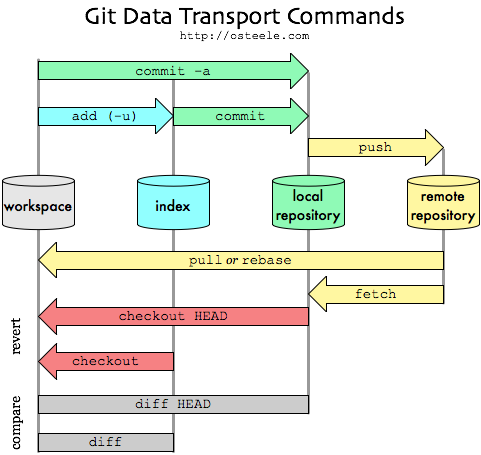
\includegraphics[scale=0.4]{flujo-git}
  \end{figure}
\end{frame}

\subsection{Construíndo a historia}
\label{subsec:Historia}

\begin{frame}[fragile]
  \frametitle{Para referenciar revisións e paths}
\begin{verbatim}
	git show 5f2df0d025026aa8785bde8cb32270aea3bac570
	git show 5f2df0d
	git show HEAD
	git show HEAD~1
	git show 5e75cda..ca1fc43
	git show :/Merged
	git checkout master
	git checkout master master
	git checkout -- master
	man git-rev-parse
\end{verbatim}
\end{frame}

\begin{frame}[fragile]
  \frametitle{Para preparar bos commits}
\begin{verbatim}
	git add -p
	git add -e
	git rm
	git mv
	git diff
	.gitignore
\end{verbatim}
\end{frame}

\begin{frame}[fragile]
  \frametitle{Para rescribir a historia}
\begin{verbatim}
	git commit --amend
	git stash
	git revert
	git cherry-pick
	git rebase -i
\end{verbatim}
\end{frame}

\begin{frame}[fragile]
  \frametitle{Para traballar en paralelo}
\begin{verbatim}
	git checkout -b mybranch master~1
	git format-patch 5e75cda..ca1fc43
	git apply 0001-Upgrade-version.patch
	git remote -v
	git remote add/rm
	git push/pull
	git init --bare
	git pull --rebase
	git push origin :master
\end{verbatim}
\end{frame}

\begin{frame}
  \frametitle{Que é e como facer unha pull request}
  \begin{figure}[ht]
    \centering
    
\includegraphics[scale=0.3]{pull_request}
    \caption{http://memegenerator.net/instance/62024625}
  \end{figure}
\end{frame}

\subsection{Utilidades para review}
\label{subsec:Review}

\begin{frame}[fragile]
  \frametitle{Para investigar na historia}
\begin{verbatim}
	git log --author=Pepe
	git log -Sconsole.log
	git blame de168bf9~1 README.md
	git bisect
\end{verbatim}
\end{frame}

\begin{frame}[fragile]
  \frametitle{Configuración avanzada}
\begin{verbatim}
	git config
	.gitconfig
	alias
\end{verbatim}
\end{frame}

\begin{frame}[fragile]
  \frametitle{Hooks}
\begin{verbatim}
	$ ls .git/hooks/

	applypatch-msg.sample     pre-push.sample
	commit-msg.sample         pre-rebase.sample
	post-update.sample        prepare-commit-msg.sample
	pre-applypatch.sample     update.sample
	pre-commit.sample
\end{verbatim}
\end{frame}

\begin{frame}
  \frametitle{Un dos grandes problemas da humanidade resolto!}
  \begin{figure}[ht]
    \centering
    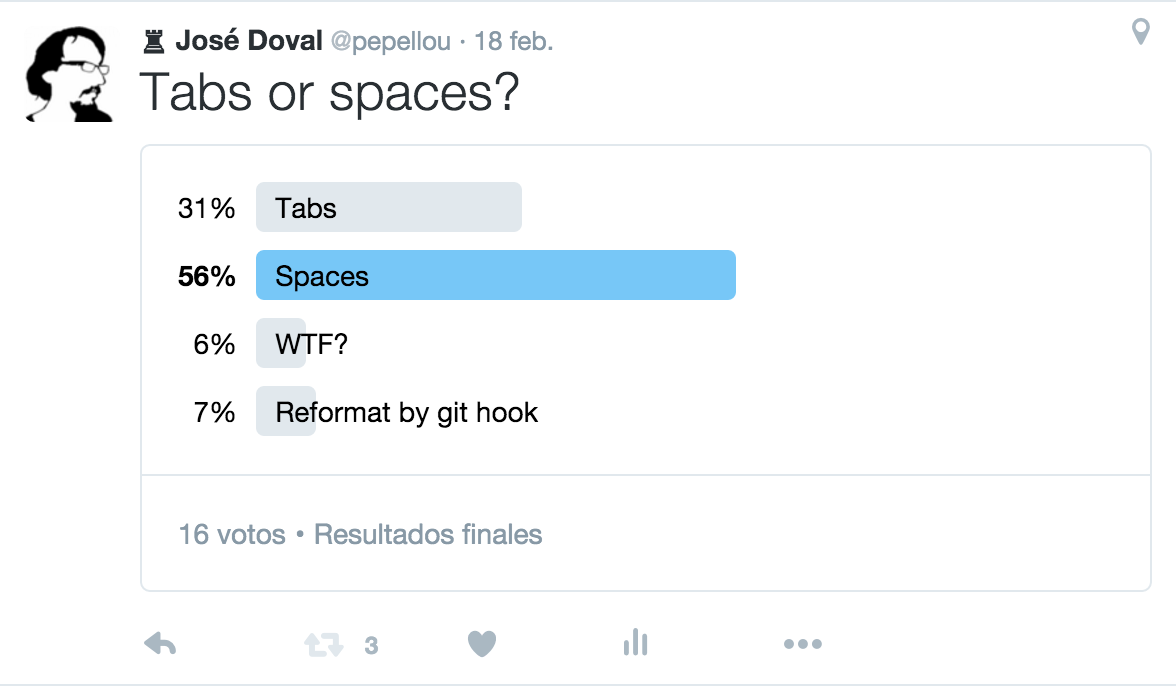
\includegraphics[scale=0.4]{tabs_vs_spaces}
  \end{figure}
\end{frame}

\subsection{Boas prácticas}
\label{subsec:BoasPracticas}

\begin{frame}
  \frametitle{Boas prácticas}
  \begin{itemize}
    \item Commits atómicos
    \item Commits frecuentes
    \item Non commitear traballo a medias
    \item Pasa os tests antes de commitear
    \item Escribe boas mensaxes de commit
    \item Usa branches, son gratis
    \item Usade todos o mesmo workflow no equipo
  \end{itemize}
\end{frame}

\begin{frame}
  \frametitle{Dúbidas?}
  \begin{figure}[ht]
    \centering
    
\includegraphics[scale=0.3]{dubidas}
    \caption{http://memegenerator.net/instance/62024625}
  \end{figure}
\end{frame}

